\begin{comment}
Problème NP vs #P
Théorème de Toda
Description du paper JVV
Complexité exacte vs approximative
Countage exact vs approximatif
Borne sur le comptage ("a tighter bound for counting max-weight solutions to 2SAT instances" ou l'équivalent pour 3SAT)
\end{comment}

\chapter{Complexité du comptage}

\begin{comment}
    \subsection*{Plan}
    
    \begin{enumerate}
        \item Introduire les problèmes algorithmiques difficiles
        \item Décrire les applications de ces problèmes
        \item Expliquer les prochaines sections
        \item Expliquer pourquoi on ne parle pas des machines de Turing (thèse de Church-Turing)
    \end{enumerate}
\end{comment}

Il est souvent favorable de décrire la théorie de la complexité à l'aide du concept de \textit{machine de Turing}. ... . Ce mémoire tentera de faire abstraction de ....


%-----------------------------------------------------------------------------%

\section{Classes de complexité}

\begin{comment}
\subsection*{Plan}

\begin{enumerate}
    \item Définir comment quantifier la complexité d'un problème (temps contre espace)
    \item Décrire le but des classes de complexité
    \item Expliquer les propriétés des classes de complexité et leurs relations
    \item Expliquer la notation de la complexité (O notation) et les machines de Turing
    \item Décrire la tour de complexité (hiérarchie polynomiale) 
    \item Comparer les classes importantes: P et NP et \#P
    \item Établir la conjecture P != NP
    \item Mentionner le théorème de Toda
    \item Parler des classes de complexités quantique
    \item Parler de la these de church-turing pour les ordis quantiques
\end{enumerate}

\subsection*{Références}

1. Moore, Cristopher, and Stephan Mertens, The Nature of Computation (Oxford, 2011; online edn, Oxford Academic, 17 Dec. 2013), https://doi.org/10.1093/acprof:oso/9780199233212.001.0001, accessed 19 July 2024.

2. Arora, S. and Barak, B. Computational Complexity: A Modern Approach. (Cambridge University Press, Cambridge, 2009). doi:10.1017/CBO9780511804090.
\end{comment}

La théorie de la complexité s'intéresse à la classification des problèmes algorithmiques en \textit{classes de complexité}, c'est-à-dire en ensembles de problèmes de même complexité. Classifier un problème permet de caractériser les ressources nécessaires pour sa résolution par un algorithme. Les problèmes d'une même classe possède une difficulté inhérente similaire, ce qui permet le choix d'un algorithme et de ressources appropriées en conséquence. Savoir qu'un problème n'est pas réalistiquement résoluble, ou plus précisément intractable, limite les attentes. Sachant ceci, la recherche dans cette direction peut s'avérer grandement utile. La théorie de la complexité cherche aussi à comparer les problèmes de différentes complexités. Ces comparaisons permettent de comprendre l'espace des problèmes en plus grande profondeur. Par exemple, il est évident que certains problèmes sont plus facile à résoudre que d'autres. Comparer des problèmes faciles avec des problèmes difficiles peut aider à comprendre ce qui rend un problème difficile et donc à trouver des algorithmes résolvant efficacement les problèmes plus complexes. Des liens, nommés réductions, peuvent aussi être définis au sein d'une même classe d'une complexité. Un algorithme efficace pour un problème pourrait aussi être efficace pour un problème similaire s'il existe une réduction entre ceux-ci. Les classes de complexité, de manière similaire au modèle de la machine de Turing, tentent de définir de manière abstraite la difficulté d'un problème. Peu importe le matériel informatique à notre disposition, un problème d'une classe donnée ne devrait pas changer de classe. Un problème trivial devrait rester trivial peu importe la quantité de ressources utilisée.  

Comment est-il possible de déterminer la complexité d'un problème? Pour ce faire, les classes de complexité se basent sur les ressources indispensables à la résolution du problème: le temps et la mémoire. Afin de trouver la solution à un problème, un programme doit effectuer un certain nombre d'opérations, limité dans le temps par le matériel informatique. On parle alors de \textit{complexité en temps}. Afin de produire un résultat final, le programme doit garder en mémoire les résultats intermédiaires. Ceux-ci doivent être sauvegardés dans le matériel informatique afin d'être réutilisés ultérieurement. Comme la quantité d'information conservée est aussi un facteur limitant pour le matériel informatique, on parle donc de \textit{complexité en espace}. 

La complexité en temps et en espace d'un problème est définie selon la taille de celui-ci. Un problème de plus grande taille est nécessairement plus complexe. \textcolor{mydarkred}{\textit{Pourquoi?}} Afin de capturer cette dépendence, on cherche à trouver une loi d'échelle encaspulant la difficulté d'un problème en fonction de sa taille. 

Le temps et la mémoire quantifient bien les ressources nécessaires des algorithmes. Par contre, ceux-ci dépendent du matériel informatique utilisé. Il est attendu qu'un ordinateur moderne soit bien plus performant qu'une des premières machines analogues. Comment retirer cette dépendence de la notion de complexité? Pour ce faire, on fait appel à la notation asymptotique, communément appelé la \textit{notation $\mathcal{O}$}. La notation asymptotique caractérise la vitesse de croissance d'une fonction en ne considérant que son comportement global à l'infini. Les coefficients ainsi que les termes asymptotiquement inférieurs ne sont pas considérés. Par exemple, pour une taille de problème $n$, la résolution de celui-ci pourrait demander un temps exponentiel $\mathcal{O}(2^{n})$ et une mémoire polynomiale $\mathcal{O}(n)$. On remarque qu'il n'y a aucune dépendence au matériel informatique: deux ordinateurs différents doivent effectuer le même nombre d'opération et sauvegarder la même quantité d'information. Un de ces ordinateurs pourraient toutefois résoudre le problème plus rapidement si celui-ci peut effectuer un plus grand nombre d'opérations par seconde ou accéder plus rapidement à sa mémoire. L'attrait des classes de complexité vient donc en partie de cette abstraction du matériel informatique.

La quantification de ces ressources permettent la séparation de plusieurs problèmes: il est en effet souhaitable d'être capable de séparer les algorithmes efficaces de ceux qui ne le sont pas. Commençons par définir deux classes de complexité particulièrement importantes: \textsf{P} et \textsf{NP}. Pour ce faire, un certain type de problème doit d'abord être défini. Un \textit{problème de décision} regroupe simplement tous les problèmes pouvant se répondre par oui ou non. Pour tout problème de décision $A$, on peut représenter celui-ci par une fonction $A(x) \in \set{ 0, 1 }$, où $x$ représente un problème particulier. Les problèmes de décision se manifestent fréquemment, tant en informatique qu'en physique. Ceux-ci se présentent sous diverses formes: Est-ce qu'un nombre $x$ est premier? La configuration $x$ représente-elle un état fondamental du système donné? Est-ce qu'il existe un chemin $x$ parcourant une seule fois toutes les villes d'une région en parcourant au maximum une distance $d$?

% \begin{maindefinition}{Problème de décision}{probleme-decision}
%     Une fonction $A(x)$ est un problème de décision si
%     \begin{align*}
%         A(x) = 
%         \begin{cases}
%            0 \text{ si } x \text{ est une réponse «non» du problème} \\
%            1 \text{ si } x \text{ est une réponse «oui» du problème}
%         \end{cases}
%     \end{align*}
% \end{maindefinition}

Quand peut-on dire qu'un problème de décision est résoluble efficacement? La classe de complexité \textsf{P}, pour «temps polynomial», tente de répondre à cette question. Informellement, un problème de la classe \textsf{P} est un problème de décision qui peut être résolu en temps polynomial. Un problème est donc considéré comme efficacement résoluble, ou \textit{tractable}, s'il appartient à la classe \textsf{P}. 

\begin{maindefinition}{Classe de complexité \textsf{P}}{classe-p}
    Une fonction $A$ fait partie de la classe de complexité \textsf{P} si et seulement si un algorithme peut calculer 
    \begin{equation*}
        A(x)=\exists y
    \end{equation*}
    en temps polynomial, c’est-à-dire en temps $O(n^{c})$ pour une taille $n = \lvert x \rvert$ et une constante $c$, où $\lvert y \rvert = \mathrm{poly}(\lvert x \rvert )$.
\end{maindefinition}

Soit, par exemple, le problème de décision du test de primalité $A$. Ce problème cherche à déterminer si un entier naturel $x$ est premier ou composé. Ce problème peut être résolu, c'est-à-dire qu'il est possible de calculer $A(x)=\exists y$, en temps polynomial $\tilde{O}(\log(n)^{12})$~\cite{PRIMESAnnalsMathematics}, où la notation $\tilde{O}$ signifie que les termes poly-logarithmiques sont aussi cachés. \textcolor{mydarkred}{\textit{Rajouter des exemples!}}

La relation entre un calcul en temps polynomial et un calcul efficace semble évidente à prime abord, comme indiqué par la thèse de Cobham–Edmonds (\textcolor{mydarkred}{\textit{Citation!}}). Cependant, certains problèmes ne possèdent pas de solutions efficaces en pratique. Par exemple, un problème peut appartenir à la classe \textsf{P}, mais être doté d'un grand coefficient limitant le calcul. Cela n'étant pas le cas pour la majorité des problèmes, cette supposition s'avère malgré tout une bonne règle empirique.

Une deuxième classe particulièrement importante en théorie de la complexité est la classe \textsf{NP}, pour «temps polynomial non-déterministe». Celle-ci regroupe les problèmes de décision dont les solutions sont vérifiables en temps polynomial. Généralement, ces problèmes sont formulés sous la forme suivante: Existe-t-il une solution, vérifiable en temps polynomial, au problème donné? Malgré que les solutions sont vérifiables efficacement, déterminer l'existence d'une telle solution n'est pas nécessairement possible en temps polynomial. Une métaphore souvent utilisée pour la description d'un problème \textsf{NP} est celle d'une aiguille dans une botte de foin. Trouver cette aiguille parmi la quantité énorme de brins de foin est un défi de taille. Par contre, une fois l'aiguille trouvée, il n'y a aucun doute qu'il s'agit bien d'une aiguille. 

\begin{maindefinition}{Classe de complexité \textsf{NP}}{classe-np}
    Une fonction $A$ fait partie de la classe de complexité \textsf{NP} si et seulement si une fonction $B \in  \textsf{P}$ existe tel que
    \begin{equation*}
        A(x) = \exists y \mid B(x,y)
    \end{equation*}
    où $\lvert y \rvert = \mathrm{poly}(\lvert x \rvert)$.
\end{maindefinition}

On appelle $B$ le vérificateur du problème de décision $A$ et $y$ le certificat ou le témoin pour l'entrée $x$. Un exemple de problème \textsf{NP} est le problème du commis voyageur. Soit un graphe $x$ représentant les villes d'un région particulière. La fonction $A$ détermine si ... \textcolor{mydarkred}{\textit{Continuer.}}
\textcolor{mydarkred}{\textit{Rajouter des exemples!}}

La classe \textsf{NP} est aussi définie comme la classe de problèmes pouvant être résolu par une machine de Turing non-déterministe en temps polynomiale, d'où son nom. Cette définition est toutefois équivalente à la définition précédente, c'est-à-dire la classe de problèmes vérifiable par une machine de Turing déterministe en temps polynomial~\cite{sipserIntroductionTheoryComputation2012}. 

\textcolor{mydarkred}{\textit{Parler de non-déterministique. Est-ce pertinent comme il faut introduire les machines de Turing non-déterministe? Autrement, un problème appartient à la classe \textsf{NP} s'il est résoluble en temps polynomial par une machine de Turing non-déterministe. }}

Notons que la classe \textsf{P} est contenue dans la classe \textsf{NP}. En effet, comme un problème de \textsf{P} est résoluble en temps polynomial, alors nécessairement une solution à ce problème peut aussi être vérifiée en temps polynomial. Cependant, une question, faisant partie des problèmes du prix du millénaire \textcolor{mydarkred}{\textit{Source?}}, demeure ouverte: est-ce que $\textsf{P} = \textsf{NP}$? La conjecture largement répandue répond à cette question par la négative. Entre autres, l'hypothèse de temps exponentiel suggère que certains problèmes de \textsf{NP} sont résolubles en temps exponentiel~\cite{impagliazzoComplexityKSAT2001}. \textcolor{mydarkred}{\textit{Conséquences?}}

\textcolor{mydarkred}{\textit{On a donc que $P \subseteq NP$.}}
\textcolor{mydarkred}{\textit{NP pour temps non-déterministique.}}
\textcolor{mydarkred}{\textit{La conjecture "Exponential Time Hypothesis" suggère que certains problèmes dans NP prennent un temps exponentiel.  (voir https://arxiv.org/pdf/1611.04471 pour plus d'information)}}

La classe de complexité d'intérêt dans le cadre de ce mémoire est la classe \textsf{\#P}. Cette classe, définie par extension à la classe \textsf{NP}, cherche non seulement à déterminer si un problème de décision possède une solution, mais aussi à spécifier le nombre de solutions à ce problème. Ainsi, un \textit{problème de comptage} consiste à trouver le nombre de solutions d'un problème de décision. Un problème de comptage est donc défini par rapport à un problème décision. Prenons par exemple le problème de décision du commis voyageur. Le problème de décision généralement défini cherche un trajet de taille inférieure à une certaine distance. Le problème de comptage adjoint exige alors le nombre de trajets possibles de taille inférieure à la distance donnée. 

\begin{maindefinition}{Classe de complexité \textsf{\#P}}{classe-sharp-p}
    Un fonction $A$ fait partie de la classe de complexité $\textsf{\#P}$ si et seulement si une fonction $B \in \textsf{P}$ existe tel que
    \begin{equation*}
        A(x) = \lvert \set{ y \mid B(x, y)} \rvert
    \end{equation*}
    où $\lvert y \rvert = \mathrm{poly}(\lvert x \rvert)$ pour toutes les valeurs $y$ prises par $B(x,y)$.
\end{maindefinition}

Par définition, un problème de la classe \textsf{\#P} est plus difficile qu'un problème de la classe \textsf{NP}. Connaître le nombre de solutions à un problème de décision indique effectivement s'il existe au moins une solution à un problème de décision.

Comme que les problèmes de la classe \textsf{P} font aussi parti de la classe \textsf{NP}, et que les problèmes de cette dernière appartiennent aussi à la classe \textsf{\#P}, il est nécessaire de définir un concept supplémentaire spécifiant la difficulté d'un problème au sein d'une classe. Intuitivement, un problème est \textit{difficile} pour une classe de complexité s'il est au moins aussi difficile que tous les problèmes de la classe. Plus formellement, un problème difficile pour une classe donnée signifie qu'il existe une \textit{réduction}, c'est-à-dire une transformation en temps polynomial d'un problème à un autre, entre ce problème et tous les autres problèmes de la classe. De plus, un problème est \textit{complet} s'il est difficile et aussi membre de la classe. La figure \textcolor{mydarkred}{\textit{Ajouter!}} éclaircit ces concepts. Les problèmes complets d'une classe représentent alors les problèmes les plus difficile de celle-ci. Par exemple, le problème du commis voyage est dit \textsf{NP}-complet, car il fait parti des problèmes considérés comme difficile de la classe \textsf{NP}. Il est toutefois crû que celui-ci ne fasse pas partie de la classe \textsf{P}.

\textcolor{mydarkred}{\textit{Parler plus en détails des réductions?}}

\begin{subtheorem}{Théorème de Toda}{toda}
    La hiérachie polynomiale \textsf{PH} est contenue dans $\textsf{P}^{\textsf{PP}}$.
\end{subtheorem}

\textcolor{mydarkred}{\textit{Définir les problèmes de décision et de comptage ainsi que les classes de complexité de manière plus formelle (alphabet, )? Changer $B(x,y)$ par $xBy$?}}

\textcolor{mydarkred}{\textit{Expliquer plus le théorème de Cook-Levin.}}

\textcolor{mydarkred}{\textit{Discuter des relations entre les classes de complexité définies.}}

\textcolor{mydarkred}{\textit{Parler des problèmes d'optimisation combinatoire.}}

\textcolor{mydarkred}{\textit{Ajouter une figure sur les classes de complexité.}}

%-----------------------------------------------------------------------------%

\section{Problème de satisfaisabilité booléenne}

\begin{comment}
\subsection*{Plan}

\begin{enumerate}
    \item Introduire SAT
    \item Énumérer certaines applications de ce problème
    \item Faire le lien entre le problème de décision SAT et le problème de comptage SAT
    \item Introduire NAE3SAT et 1in3SAT
    \item Énoncer la réduction entre NAE3SAT/1in3SAT et 3SAT
    \item Introduire la transition de phase critique de ces problèmes
    \item Expliquer pourquoi prendre la version positive de ces problèmes n'est pas un problème
    \item Parler du comptage des problèmes SAT
    \item Introduire la transition de phase critique de ces problèmes
\end{enumerate}

\subsection*{Références}

1. Moore, Cristopher, and Stephan Mertens, The Nature of Computation (Oxford, 2011; online edn, Oxford Academic, 17 Dec. 2013), https://doi.org/10.1093/acprof:oso/9780199233212.001.0001, accessed 19 July 2024.

2. Arora, S. and Barak, B. Computational Complexity: A Modern Approach. (Cambridge University Press, Cambridge, 2009). doi:10.1017/CBO9780511804090.

3. Achlioptas, D., Chtcherba, A., Istrate, G. and Moore, C. The phase transition in 1-in-k SAT and NAE 3-SAT. Proceedings of the Annual ACM-SIAM Symposium on Discrete Algorithms (2001) doi:10.1145/365411.365760.
\end{comment}

Le problème de \textit{satisfaisabilité booléenne}, ou problème SAT est particulièrement important dans la théorie de la complexité. Montré comme \textsf{NP}-complet par le théorème de Cook-Levin~\cite{cookComplexityTheoremprovingProcedures1971,levinUniversalSequentialSearch}, il fut à la base de la définition de \textsf{NP}-complétude et du problème $\textsf{P} = \textsf{NP}$. Celui-ci est aussi couramment utilisé dans la preuve de réductions de problèmes au sein de la classe de complexité \textsf
{NP} \textcolor{mydarkred}{\textit{Rajouter des sources.}}. Le problème SAT a une multitude d'applications, comme \textcolor{mydarkred}{\textit{Rajouter des exemples.}}, en partie grâce à la facilité de formuler ces applications à l'aide de formules propositionnelles.

Une \textit{formule propositionnelle}, ou une expression booléene, est un ensemble de variables booléenes, $x_{i} \in \set{ 0, 1 }$, reliées par des opérateurs booléeans de conjections ("ou", $\lor$), de disjonctions ("et", $\land$) ainsi que de négation ("non", $\neg$). Un \textit{litéral} désigne dans ce contexte une variable booléene ou sa négation. Par exemple, l'expression $(x_{1} \land x_{2}) \lor \neg x_{3}$ est une formule booléenne composée des variables $x_{1}$, $x_{2}$ et $x_{3}$, ainsi que des littéraux $x_{1}$, $x_{2}$ et $\neg x_{3}$. 

Un problème SAT se décrit par une formule propositionnelle. Résoudre le problème consiste à déterminer s'il existe une combinaison de variables qui rend la formule logiquement vraie, c'est-à-dire tel que l'évaluation de celle-ci donne 1. Une telle formule est alors dite satisfaisable.

\begin{maindefinition}{Problème SAT}{probleme-sat}
    Soit une constante $n \geq 1$ et une formule propositionnelle $\varphi(x_{1}, x_{2}, \dots, x_{n})$ où $x_{i} \in \set{ 0, 1 }$.  Existe-il une assignation des variables $x_{1}, x_{2}, \dots, x_{n}$ telle que $\varphi$ soit satisfaisable, c'est-à-dire que $\varphi(x_{1}, x_{2}, \dots, x_{n})=1$?
\end{maindefinition}

Dans l'étude du problème SAT, les formules propositionnelles sont souvent exprimées en \textit{forme normale conjonctive} (« Conjunctive Normal Form ») (CNF). On parle alors de formules CNF. Celles-ci consiste en une conjonction d'une ou de plusieurs \textit{clauses}, où une clause est une disjonction d'un ou plusieurs littéraux. Cela implique que toute clause doit contenir au moins un littéral évaluant à 1 pour que la formule soit satisfaisable. Toute formule propositionnelle peut être réécrite en forme normale conjonctive en utilisant les lois de l'algèbre booléenne.

\begin{example}{Problème SAT}{probleme-sat}
    La formule CNF
    \begin{equation*}
        \varphi(x_{1}, x_{2}, x_{3}) = (x_{1} \lor x_{3}) \land (\neg x_{1} \lor x_{2} \lor \neg x_{3}) 
    \end{equation*}
    est satisfaisable car $\varphi(1,0,0) = (1 \lor 0) \land (\neg 1 \lor 0 \lor \neg 0) = 1$. Au contraire, la formule CNF
    \begin{equation*}
        \varphi(x_{1}, x_{2})= (x_{1}) \land (\neg x_{1})
    \end{equation*}
    n'est pas satisfaisable car $\varphi (x_{1}) = 0$ peu importe le choix de $x_{1}$.
\end{example}

Un cas spécial du problème SAT est le problème kSAT, où le nombre de littéraux appartenant à chaque clause d'une formule CNF est restreint à $k$ littéraux au maximum. Notons que le problème kSAT est trivial pour $k=1$, résoluble en temps linéaire pour $k=2$, et \textsf{NP}-complet pour $k \geq 3$ \textcolor{mydarkred}{\textit{Source?}}.

Dans ce mémoire, deux variantes de 3SAT seront portées à l'étude: le problème Pas-Tous-Égaux 3SAT (« Not-All-Equal 3-Satisfiability ») (NAE3SAT) et le problème 1-dans-3 3SAT (« One-in-three 3-Sastisfiability ») (1-in-3SAT).

\begin{maindefinition}{Problème NAE3SAT}{probleme-nae3sat}
    SoSoit une formule CNF $\varphi(x_{1}, x_{2}, \dots, x_{n})$ pour laquelle chaque clause $C$ contient au maximum 3 littéraux. Existe-il une assignation des variables $x_{1}, x_{2}, \dots, x_{n}$ telle que $\varphi$ soit satisfaisable tout en s'assurant que toutes les littéraux de chaque clause $C$ ne soit pas égales?
\end{maindefinition}

Notons qu'un problème NAE3SAT peut être réduit à un problème 3SAT. Soit $f$ une formule CNF représentant un problème 3SAT. Dans ce cas, la formule $g = f \land \neg f$ décrit le problème NAE3SAT associé.

\begin{maindefinition}{Problème 1-in-3SAT}{probleme-1in3sat}
    Soit une formule CNF $\varphi(x_{1}, x_{2}, \dots, x_{n})$ pour laquelle chaque clause $C$ contient au maximum 3 littéraux. Existe-il une assignation des variables $x_{1}, x_{2}, \dots, x_{n}$ telle que $\varphi$ soit satisfaisable tout en s'assurant qu'exactement un littéral de chaque clause $C$ soit logiquement vrai?
\end{maindefinition}


Les précédents problèmes de décision peuvent être associés à des problèmes de comptage: \#NAE3SAT et \#1-in-3SAT. 


%-----------------------------------------------------------------------------%

\section{Intractabilité et approximations}

\begin{comment}
\subsection*{Plan}

\begin{enumerate}
    \item Expliquer le concept d'intractabilité
    \item Montrer la difficulté de résoudre des problèmes computationnels de manière exacte
    \item Expliquer les advantages des méthodes approximatives (temps polynomial, applications réelles)
    \item Introduire rigoureusement le concept d'approximation
\end{enumerate}

\subsection*{Références}

Subhash Khot. Inapproximability of NP-complete Problems, Discrete Fourier Analysis, and Geometry. In Proceedings of the International Congress of Mathematicians 2010 (ICM 2010)
\end{comment}



%-----------------------------------------------------------------------------%

\section{Complexité et bornes sur le comptage}

\subsection*{Plan}

\begin{enumerate}
    \item Décrire les résultats actuels en terme de comptage exact et approximatif
    \item Énumérer les algorithmes et les solveurs modernes (DPLL, \textit{survey propagation}, \textit{belief propagation})
    \item Mentionner les meilleures bornes sur les problèmes de comptage
    \item https://arxiv.org/pdf/2002.06879
    \item Lien avec la fonction de partition
\end{enumerate}


\subsection*{Références}

1. Wahlström, M. A Tighter Bound for Counting Max-Weight Solutions to 2SAT Instances. in Parameterized and Exact Computation (eds. Grohe, M. and Niedermeier, R.) 202–213 (Springer, Berlin, Heidelberg, 2008). doi:10.1007/978-3-540-79723-419.

2. Sinclair, A. and Jerrum, M. Approximate counting, uniform generation and rapidly mixing Markov chains. Information and Computation 82, 93–133 (1989).


%-----------------------------------------------------------------------------%

\section{Transitions de phase}

\begin{comment}
\subsection*{Plan}

\begin{enumerate}
    \item Expliquer les différentes transitions de phase et leurs intuitions
    \item Décrire l'objectif des algorithmes classiques locaux et globaux, comme le "belief propagation" ou le "survey propagation"
    \item Expliquer brièvement où se situe VQCount par rapport à ça
\end{enumerate}

\subsection*{Références}

1. Watrous, J. Quantum Computational Complexity. Preprint at https://doi.org/10.48550/arXiv.0804.3401 (2008).

2. Mézard, M. and Montanari, A. Information, Physics, and Computation. (Oxford University Press, Oxford, New York, 2009).

2. https://www.sciencedirect.com/science/article/pii/S0378437109010656

3. Survey propagation: An algorithm for satisfiability - Braunstein - 2005 - Random Structures amp; Algorithms - Wiley Online Library. https://onlinelibrary.wiley.com/doi/abs/10.1002/rsa.20057.
\end{comment}

La complexité d'une instance aléatoire d'un problème \textsf{NP} n'est pas toujours identique. En réalité, certaines instances sont résolubles en temps polynomial, alors que d'autres sont intractables. Les discussions autour des classes de complexité s'intéressent principalement à la complexité dans le pire des cas pour décrire la difficulté inhérente d'un problème. Cependant, certaines instances peuvent posséder une complexité inférieure, pouvant alors être pris en avantage par certains algorithmes. 

Pour les problèmes SAT, la difficulté d'une instance aléatoire est grandement dépendante sur le ratio du nombre de clauses $C$ sur le nombre de variables $v$. Plus surprenamment, ce ratio $\alpha = \frac{\#c}{\#v}$ est un indicateur d'une transition de phase de la complexité du problème SAT. En effet, il existe une valeur critique $\alpha_{c}$ où les instances du problème SAT passe de satisfaisable à insatisfaisable. La difficulté du problème SAT semble provenir juste avant cette transition.

Plusieurs autres transitions de phase existent avant la transition critique. 

\begin{figure}[h]
    \centering
    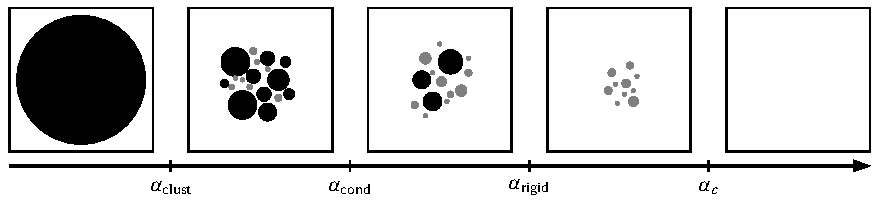
\includegraphics[width=1\textwidth]{figures/phase-transitions.pdf}
    \caption{}
    \label{fig:...}
\end{figure}